\begin{question}
\noindent Triangle $T$ has vertices $A(1,1)$, $B(3,1)$ and $C(1,3)$, as shown on the grid.

\begin{center}
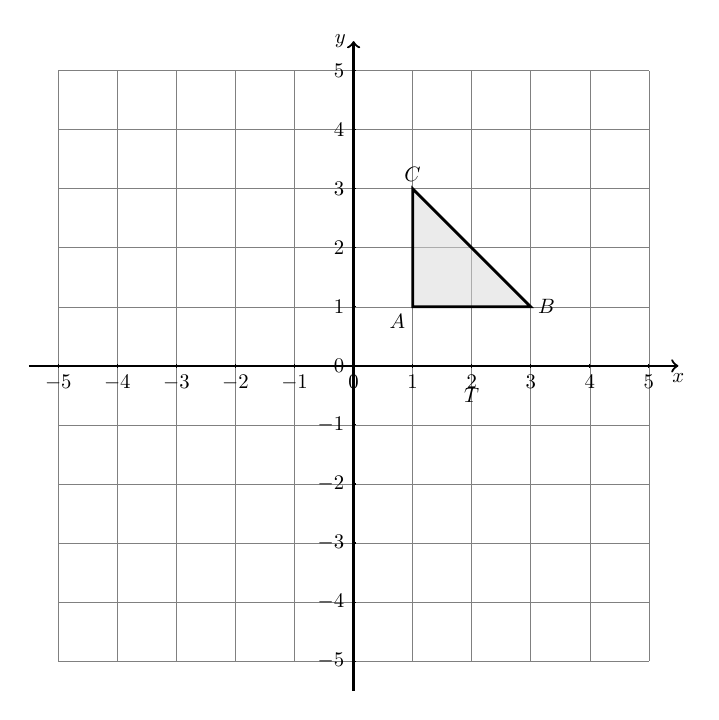
\begin{tikzpicture}[scale=0.75, transform shape]
    % Define colours
    \definecolor{borderColour}{HTML}{000000}
    \definecolor{fillColour}{HTML}{D8D8D8}

    % Define axis scale
    \def\axisLimit{5}

    % Draw grid
    \draw[step=1cm,gray,very thin] (-\axisLimit,-\axisLimit) grid (\axisLimit,\axisLimit);

    % Draw axes
    \draw[thick,->] (-\axisLimit-0.5,0) -- (\axisLimit+0.5,0) node[anchor=north] {$x$};
    \draw[thick,->] (0,-\axisLimit-0.5) -- (0,\axisLimit+0.5) node[anchor=east] {$y$};

    % Label x-axis
    \foreach \x in {-\axisLimit,...,\axisLimit}
        \draw (\x cm,1pt) -- (\x cm,-1pt) node[anchor=north] {$\x$};
    % Label y-axis
    \foreach \y in {-\axisLimit,...,\axisLimit}
        \draw (1pt,\y cm) -- (-1pt,\y cm) node[anchor=east] {$\y$};

    % Define coordinates for triangle T
    \coordinate (A) at (1,1);
    \coordinate (B) at (3,1);
    \coordinate (C) at (1,3);

    % Draw triangle T
    \filldraw[fill=fillColour, draw=borderColour, line width=1pt, fill opacity=0.5] (A) -- (B) -- (C) -- cycle;

    % Label the vertices
    \node[below left] at (A) {$A$};
    \node[right] at (B) {$B$};
    \node[above] at (C) {$C$};

    \node at (2,-0.5) {$T$};

\end{tikzpicture}
\end{center}

\noindent Triangle $T$ is a Valorant map designer's blueprint tile that must go through two transformations before it is placed onto the final map layout.

\begin{enumerate}
    \item[(a)] Reflect triangle $T$ in the line $y = 0$ (the $x$-axis) to give triangle $U$.

    Find the coordinates of the vertices of triangle $U$.
    \vspace{4cm}
    \answerplain{2}

    \item[(b)] Triangle $U$ is then rotated $90^\circ$ clockwise about the origin $O$ to give triangle $V$.

    Find the coordinates of the vertices of triangle $V$.

    \noindent \textbf{Warning:} A student who rotates triangle $T$ first, then reflects it, will not get the correct final answer for $V$ --- the transformations must be applied to $U$, in the order given.
    \vspace{4cm}
    \answerplain{2}
\end{enumerate}
\end{question}
